%---------------------------------------------------------------------------------------%	SECTION 4.1

%---------------------------------------------------------------------------------------

\section{The Riemann Integral.}

\begin{definition}
    Let $a,b \in \R$, with  $a<b$. We define a  \textbf{partition} of $[a,b]$ to be a set of points $P=\{x_0,x_1, \dots, x_n\}$ such that $a=x_0<x_1< \dots <x_n=b$.
    We define the \textbf{norm} of a partion $P=\{x_0,x_1, \dots, x_n\}$ to be the number:
    \begin{equation}
        ||P||=\max|x_j-x_{j-1}|
    \end{equation} 
    We call a \textbf{refiment} of a partition $P=\{x_0,x_1, \dots, x_n\}$ to be a partition $Q$ of  $[a,b]$ such that  $P \subseteq P$, and we say that $Q$ is  \textbf{finer} than $P$. We say that $P$ and  $Q$ are  \textbf{noncomparable} if neither is a refinment of the other if neither is a refinment of the other..
\end{definition}

\begin{example}[Dyadic Partitions]
    Let $P_n=\{\frac{j}{2^n}: j=0,1, \dots 2^n\}$, then $P_n$ is a partiton of  $[0,1]$, and  $P_m$ is finer than  $P_n$ if  $m>n$.
    Dyadic are good choices for partitions.
\end{example} 

If we have two partitions $P$ and  $Q$, in general, they may have no relation. But, $P \cup Q$ is a refinment of both  $P$ and  $Q$. Now if  $Q$ is finer than $P$, we see that  $||Q|| \leq ||P||$, that is the norm is a monotonically decreasing function of  $x_j$.

\begin{figure}
    \centering
    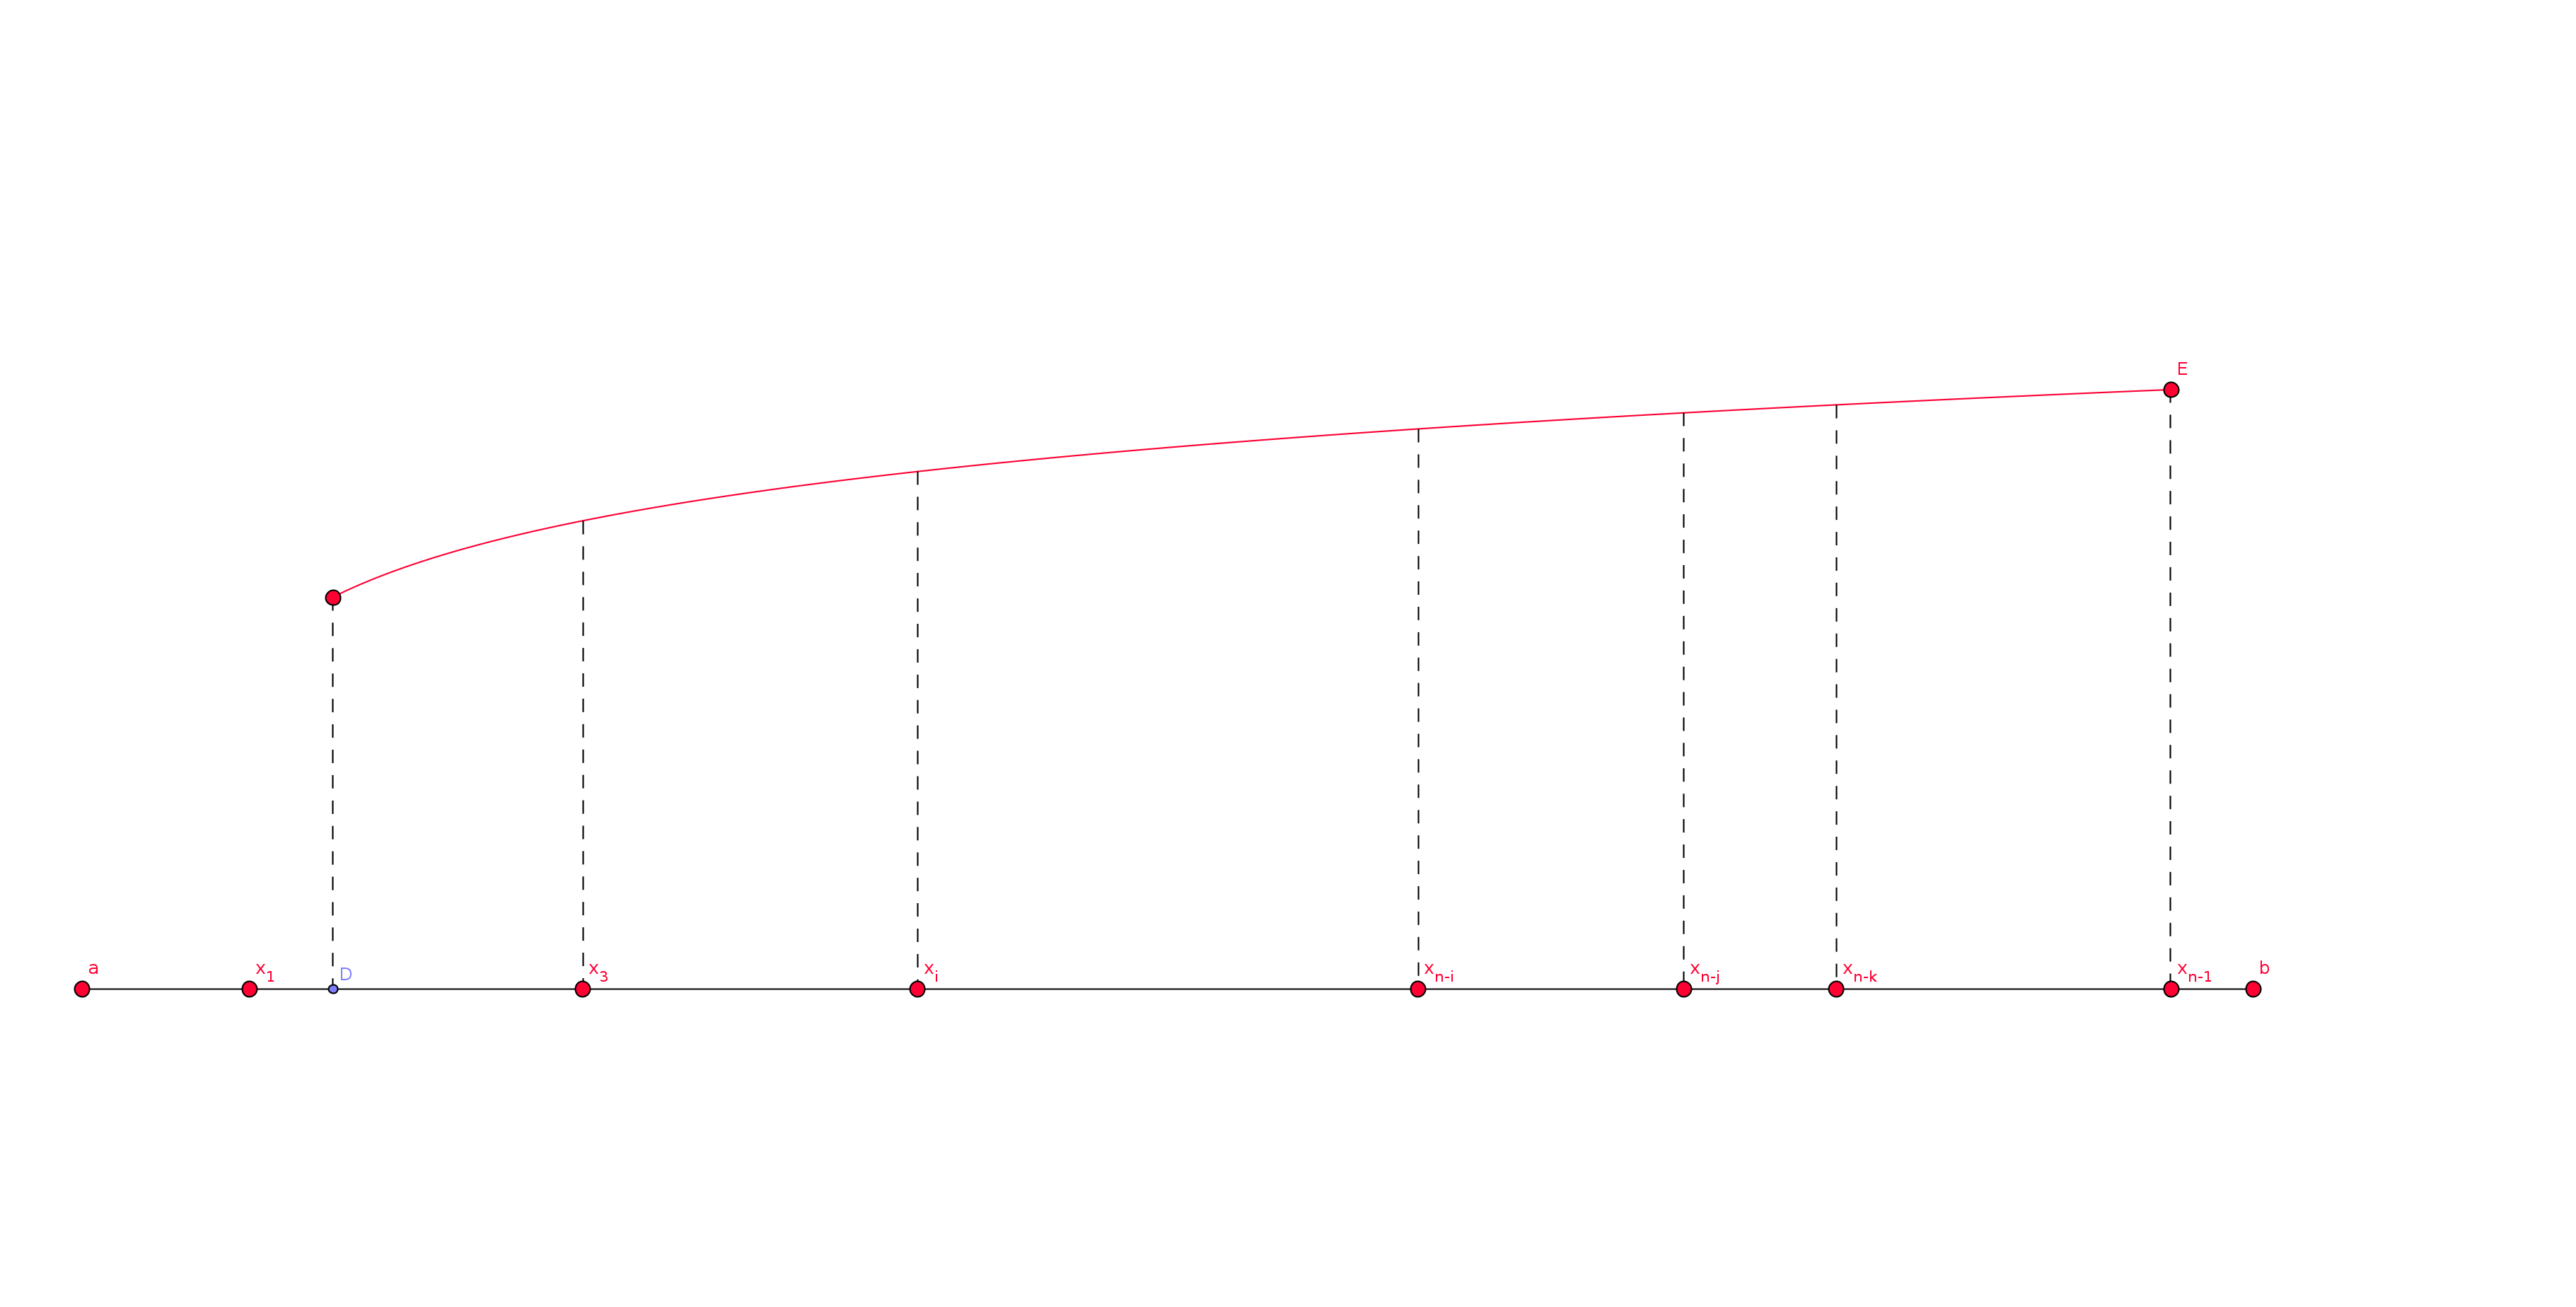
\includegraphics[scale = 0.5]{figures/partitionOfACurve.png}
    \caption{The Riemann Sum of a nonnegative bounded curve over the interval $[a,b]$.}
    \label{fig_5.1}
\end{figure}

\begin{definition}
    Let $a,b \in \R$ with  $a<b$ let $P=\{x_0,x_1, \dots, x_n\}$ be a partition of  $[a,b]$, and suppose that  $f:[a,b] \rightarrow \R$ is bounded. 
    We define the  \textbf{upper Riemann sum} of $f$ over  $P$ to be:
     \begin{equation}
         U(f,P)=\sum_{j=1}^{n}{M_j(f)(x_j-x_{j-1})}		
    \end{equation} 
    where $M_j(f)=\sup{f(x)}$ where  $x \in [x_{j-1},x_j]$.

We define the \textbf{lower Riemann sum} of $f$ over  $P$ to be:
     \begin{equation}
         L(f,P)=\sum_{j=1}^{n}{m_j(f)(x_j-x_{j-1})}
    \end{equation}
    Where $m_j(f)=\inf{f(x)}$ with  $x \in [x_{j-1},x_j]$
\end{definition}

\begin{remark}
    SUppose that $f(x)=\alpha$ is a constant function on  $[a,b]$. Then  $M_j(f)=m_j(f)=\alpha$, hence we see that
        \begin{equation*}
            U(f,P)=L(f,P)=\alpha\sum_{j=1}^{n}{x_j-x_{j-1}}=\alpha(b-a)
        \end{equation*} 
\end{remark}

\begin{remark}
    We have that $L(f,P) \leq U(f,P)$ for all  partitions $P$ and bounded functions  $f$, since $\inf{f} \leq \sup{f}$, so the relevant equalities follow.
\end{remark}

\begin{lemma}\label{5.1.1}
    If $P$ is any partition of  $[a,b]$, and there is a refinment of $P$, $Q$, then $L(f,P) \leq L(f,Q) \leq U(f,Q) \leq U(f,P)$. 
\end{lemma}
\begin{proof}
    Assume that $Q=P \cup \{x'\}$, with $x_{j-1}<x'<x_j$.
    Then $L(f,P)=\sum{m_j(f)(x_j-x_{j-a})}+m_j(f)(x_j-x'+x'-x_{j-1}) \leq \sum{m_j(f)(x_j-x_{j-1})}+m_{j_0'}(f)(x_{j_0}-x')+m_{j_0''}(f)(x'-x_j_0)=L(f,Q)$. We see that $inf{f}$ is increasing while $\sup{f}$ is decreasing, hence we get that  $U(f,Q) \leq U(f,P)$ by similar reasoning, and clearly  $L(f,Q) \leq U(f,Q)$.
\end{proof}
\begin{remark}
    What lemma \ref{5.1.1} says is that the lower sum is monotonically increasing while the upper sum is monotonically decreasing with respect to the refinment.
\end{remark}

\begin{lemma}\label{5.1.2}
    If $P$ and  $Q$ are any partitions of  $[a,b]$, then  $L(f,P) \leq U(f,Q)$.
\end{lemma}
\begin{proof}
    For refinment, lower sums are monotonically increasing, and upper sums are monotonically decreasing, and the result follows from lemma \ref{5.1.1}. Now suppose that $P$ and  $Q$ are noncomparable. Now $P \cup Q$ is a refinment of both  $P$ and  $Q$, hence, by direct application of lemma \ref{5.1.1}, we have $L(f,P) \leq L(f,P \cup Q) \leq U(f,P \cup Q) \leq U(f,Q)$.
\end{proof}
\begin{remark} 
    Now we have that with respect to refinment, we have that all upper sums are bounded below, and all lower sums are bounded above, hence the least upper, and greates lower bounds are finite and exist.
    now when they apporach a certain value, we we obtain the ``integral'' of $f$ with  over the interval $[a,b].$
\end{remark}

\begin{definition}
    Let $a,b \in \R$, with  $a<b$ a realvalued function $f:[a,b] \rightarrow \R$ is said to be \textbf{Riemann integrable} (or \textbf{integrable}) on $[a,b]$ if and only if  $f$ is bounded on  $[a,b]$, and for every  $\epsilon>0$, there is a partition  $P$ of $[a,b]$ such that  $U(f,p)-L(f,P)<\epsilon$.
\end{definition}

\begin{theorem}\label{5.1.3}
    Suppose that $a,b \in \R$, with  $a<b$. If  $f$ is continuous on  $[a,b]$, then  $f$ is integrable on  $[a,b]$.
\end{theorem}
\begin{proof}
    We know that if a function is continuous over a closed interval, then it is uniformly continuous.
    Given  $\epsilon>0$, we have that  $f$ is uniformly continuous over  $[a,b]$, then there is a  $\delta>0$ such that $|f(x)-f(y)|<\frac{\epslon}{b-a}\epslon$ whenever $|x-y|<\delta$, for  $x,y \in [a,b]$.
    Let $P=\{x_0,x_1, \dots, x_n\}$ be a partition of $[a,b]$, with  $||P||<\delta$. For the  $j$th subinterval, by the extreme value theorem, tehre are $x_m, x_M \in [x_{j-1},x_j]$ with $m_j(f)=f(x_m)$ and  $M_j(f)=f(x_M)$.
    Now  $|x_M-x_m|<\delta$, so  $|f(x_M)-f(x_m)|=M_j(f)-m_j(f)<\frac{\epsilon}{b-a}$.
    Then we have:
        \begin{equation*}
            U(f,P)-L(f,P)=\sum{M_j(f)-m_j(f)(x_j-x_{j-1})} \leq \sum{\frac{\epsilon}{b-a}}=\frac{\epsilon}{b-a}(b-a)=\epsilon
        \end{equation*} 
hence, $f$ is integrable.
\end{proof}

\begin{example}
    \begin{enumerate}[label=(\arabic*)]
        \item The Dirichlet function, $f(x)=\begin{cases}
                1 & x \in \Q \\
                0 & x \notin \Q \\
            \end{cases}$
            is not Riemann integrable on $[0,1]$.
            Choose $P=\{x_0,x_1 \dots , x_n\}$ a partition of $[0,1]$, for  $[x_j,x_{j-1}]$, we have  $M_j(f)=1$ and  $m_j(f)=0$ by definition of  $f$. Then  $U(f,P)-L(f,P)=\sum{1 \cdot (x_j-x_{j-1})}+\sum{0 \cdot (x_j-x_{j-1})}=\sum{(x_j-x_{j-1})}=1$, hence.

    \item Constant functions are always Riemann integrable.

    \item Let $f(x)=\begin{cases}
            0 & 0 \leq x<\frac{1}{2} \\
            1 & \frac{1}{2} \leq x \leq 1
        \end{cases}$.
        Now given $\epsilon>0$, construct  $P=\{0,\frac{1-\epsilon}{2},\frac{1+\epsilon}{2},1\}$ for $\epsilon<\frac{1}{2}$. Then:
        \begin{equation}
            U(f,P)-L(f,P)= 1 \cdot (\frac{1+\epsilon}{2}-\frac{1-\epsilon}{2})=\epsilon		
        \end{equation} 
        So, we have that $f$ is integrable is integrable.
    \end{enumerate}
\end{example} 

\begin{definition}		
    Let $a,b \in \R$ with  $a<b$, and let  $f:[a,b] \rightarrow \R$ be a realvalued function.
    We define the \textbf{upper Riemann intergral} of $f$ over  $[a,b]$ to be:
        \begin{equation}
            \bar{\int_{a}^{b}}{f(x) dx}=\inf\{U(f,P):P \text{ is a partition of } [a,b]\}. 
        \end{equation}
    Similarly, we define the \textbf{lower Riemann integral} of $f$ over  $[a,b]$ to be:
        \begin{equation}
            \bbar{\int_{a}^{b}}{f(x) dx}=\sup\{U(f,P):P \text{ is a partition of } [a,b]\}. 
        \end{equation} 
        Lastly, if $\bar{\int_{a}^{b}}{f}=\bbar{\int_{a}^{b}}{f}$, then we define the \textbf{Riemann Integral} to be:
        \begin{equation}
            \int_{a}^{b}{f(x) dx}=\bar{\int_{a}^{b}}{f(x) dx}=\bbar{\int_{a}^{b}}{f(x) dx}
        \end{equation}
        Now if $a=b$, we define  $\int_{a}^{b}{f}=0$ for all bounded functions  $f$. If $b<a$, we define  $\int_{a}^{b}{f}=-\int_{b}^{a}{f}$.
\end{definition}

Now not all bounded functions may be integrable, however, the lower and upper Riemann integrals always exist.

\begin{lemma}\label{1.5.4}
    $\bbar{\int_{a}^{b}}{f} \leq \bar{\int_{a}^{b}}{f}$.
\end{lemma}
\begin{proof} 		
    Applying lemma \ref{5.1.2}, we have $L(f,P) \leq U(f,Q)$, now  $L(f,P)$ is a lowerbound of all uppersums, hence  $L(f,P) \leq \bar{\int_{a}^{b}}{f}$.
    Now $L(f,P) \leq \bar{\int_{a}^{b}}{f}$ is an upperbound of all lowersums, hence $\bbar{\int_{a}^{b}}{f} \leq \bar{\int_{a}^{b}}{f}$
\end{proof}

\begin{theorem}\label{5.1.5}
    Let $a,b \in \R$ with  $a<b$, and let  $f:[a,b] \righarrow \R$ be a bounded realvalued function.
    Then  $f$ is integrable on  $[a,b]$ if and only if  $\bbar{\int_{a}^{b}}{f}=\bar{\int_{a}^{b}}{f}$.
\end{theorem}
\begin{proof}
    Suppose thay $f$ is integrable, then for  $\epsilon>0$, there is a partition  $P$ such that  $U(f,P)-L(f,P) \leq \epsilon$ whenever  $||P|| \leq \delta$.
    Noq we have that $L(f,) \leq \bbar{\int_{a}^{b}}{f} \leq \bar{\int_{a}^{b}}{f} \leq U(f,P)$.
    So  $\bar{\int_{a}^{b}}{f}-\bbar{\int_{a}^{b}}{f} \leq U(f,P)-L(f,P)<\epsilon$. Hence  $\bar{\int_{a}^{b}}{f}-\bbar{\int_{a}^{b}}{f}=0$.

    Conversely, suppose that $\bar{\int_{a}^{b}}{f}-\bbar{\int_{a}^{b}}{f}=0$, then given $\epsilon>0$, there is a partition  $P_1$ of  $[a,b]$, with:
        \begin{equation*}
             \bar{\int_{a}^{b}}{f} \leq U(f,P)<	\bar{\int_{a}^{b}}{f}+\frac{\epsilon}{2}
        \end{equation*}
Likewise, there is a partition $P_2$ of $[a,b]$ with:
        \begin{equation*}
            \bbar{\int_{a}^{b}}{f}-\frac{\epsilon}{2}<U(f,P) \leq \bbar{\int_{a}^{b}}{f}
        \end{equation*}
        Now let $P=P_1 \cup P_2$, then:
        \begin{equation*}
            \bar{\int_{a}^{b}}{f}-\bbar{\int_{a}^{b}}{f}{2}<U(f,P)-L(f,P)<\bar{\int_{a}^{b}}{f}-\bbar{\int_{a}^{b}}{f}<\frac{\epsilon}{2}+\frac{\epsilon}{2}=\epsilon
        \end{equation*}.
        Hence, $f$ is integrable over  $[a,b]$.
\end{proof}

\begin{theorem}\label{5.1.6}
    If $f(x)=\alpha$ is a constant function on  $[a,b]$, then  $\int_{a}^{b}{f(x) dx}=\alpha(b-a)$ for all  $x \in [a,b]$.
\end{theorem}
\begin{proof}
    We have that $f$ is integrable, so  $\bar{\int_{a}^{b}}{f}=\bbar{\int_{a}^{b}}{f}$, moreover we have  $U(f,P)=L(f,P)=\alpha(b-a)$, combining these two, we get the desired result.
\end{proof}
